\chapter{介绍}
	在数据中查找模式的问题是一个基础性问题,并且有很长而成功的历史。例如,Tycho Brahe在16世纪广泛的天文观察是的开普勒发现了天体运动规律,这又提供了经典力学发展的跳板。同样的,原子光谱规律的发现也对量子物理的发展和验证起到了关键的作用。模式识别领域关注于使用计算机算法来自动地发现数据中的规律,并且使用这些规律进行如对不同类别进行分类的一些活动。
	
	思考手写数字的识别例子,如图1.1。每个数字对应$28 \times 28$个像素,可以使用包含784个实数的向量$\mathbf{x}$来表示。目标是去构建一个机器,向量$\mathbf{x}$作为输入,产生数字$0,\dots, 9$作为输出。可以使用手工规则或者启发式来根据笔画形状来区分数字,但是这种方法在实践中会导致增加例外的规则,并且不约而同地给出糟糕的结果。
	
\begin{figure}
	\centering
	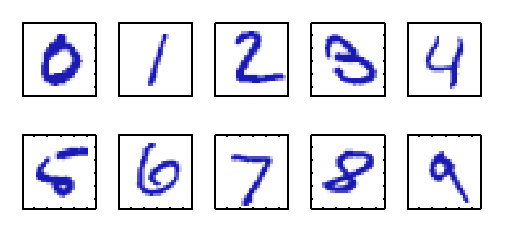
\includegraphics[width=8cm]{Figure1-1.eps}
	\caption{Examples of hand-written digits taken from US zip codes} 
	\label{fig:endb-flow} 
\end{figure}

	更优的结果是采用机器学习方法,这种方法中有一个很大的数字集合N $\{ \mathbf{x_1},$ $ \dots, \mathbf{x_N} \}$ 称为训练集,用来调整得到可适应模型的参数。在训练数据集中的数字分类已经提前给出,通常通过单独手工贴标签来检查他们。我们可以使用目标向量$\mathbf{t}$来表达一个数字的分类,表示对应数字的定义。对于用向量来表示的类别技术会在后面来进行讨论。注意到这里对于每一个数字图像$\mathbf{x}$,使用一个目标向量来表示。
	
	机器学习算法运行的结果可以表示为一个函数$\mathbf{y(x)}$,函数使用一个新的数字图像$\mathbf{x}$作为属兔,产生一个输出向量$\mathbf{y}$,其和目标向量的编码相同。函数$\mathbf{y(x)}$的精确格式在基于训练数据训练阶段时候确定,也被称作学习阶段。当模型确定后,就可以用来确定一个新的的数字图像,包括一个测试数据集。新样本的分类正确性不同于用来训练数据样本的能力称作一般化(generalization)。在实践应用中,
\section{图模型}

